\documentclass{standalone}
\usepackage{tikz}
\usetikzlibrary{matrix, arrows.meta}

\begin{document}

\[
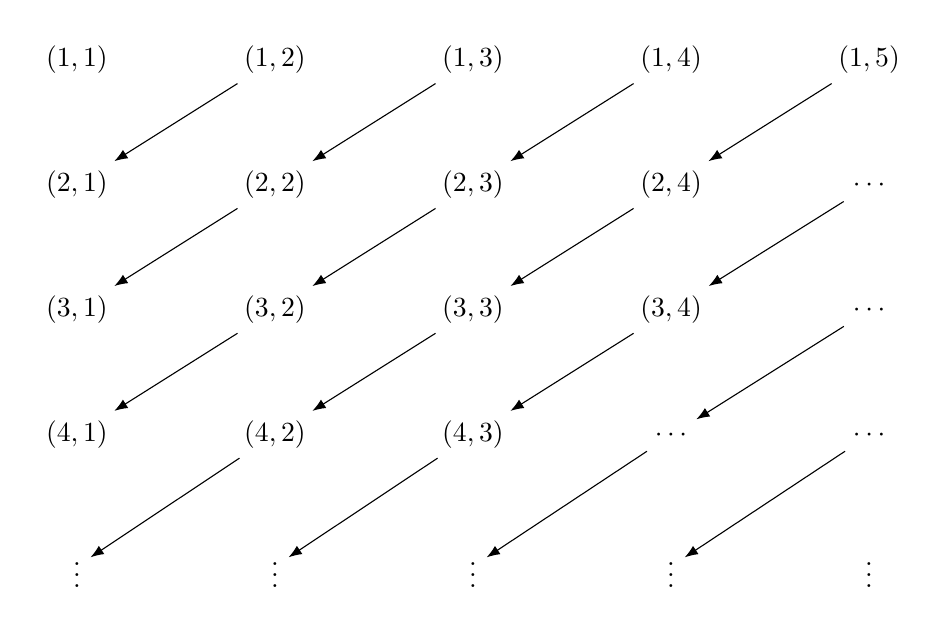
\begin{tikzpicture}[>=Latex]
\matrix[matrix of math nodes, row sep=1cm, column sep=1.5cm] (m) {
(1,1) & (1,2) & (1,3) & (1,4) & (1,5) \\
(2,1) & (2,2) & (2,3) & (2,4) & \cdots \\
(3,1) & (3,2) & (3,3) & (3,4) & \cdots \\
(4,1) & (4,2) & (4,3) & \cdots & \cdots \\
\vdots & \vdots & \vdots & \vdots & \vdots \\
};

% Draw arrows diagonally down-left: from (i,j) to (i+1,j-1)
\foreach \i in {1,2,3,4} {
  \foreach \j in {2,3,4,5} {
    \pgfmathtruncatemacro{\ii}{\i + 1}
    \pgfmathtruncatemacro{\jj}{\j - 1}
    \ifnum\ii<6
      \draw[->] (m-\i-\j) -- (m-\ii-\jj);
    \fi
  }
}

\end{tikzpicture}
\]

\end{document}